%pictures and spectra
%tables and graphs
%statements of the result

%%% three subfigures next to each others
% \begin{figure*}
%     \centering
% \begin{subfigure}{.3\textwidth}
%     \centering
%     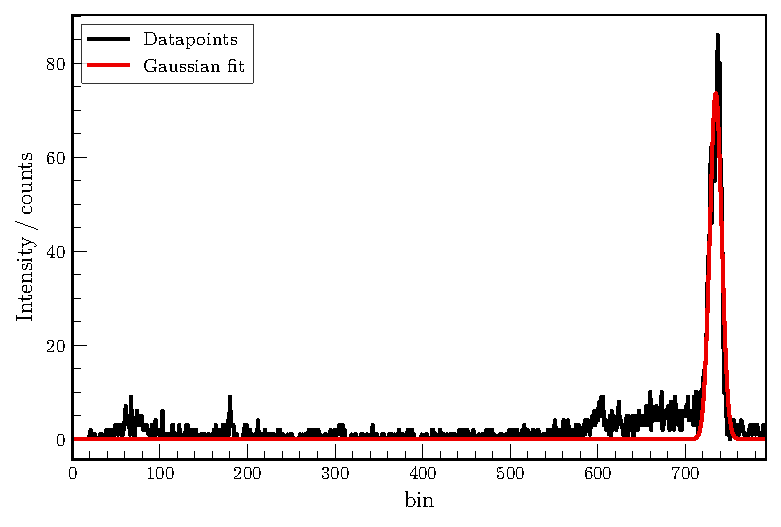
\includegraphics[width=\textwidth]{plots/source-spectrum.pdf}
%     \caption{Spectrum of the source $\ce{Cs}$ due to the decay of $\ce{Br}$. }
% \end{subfigure}
% \begin{subfigure}{.3\textwidth}
%     \centering
%     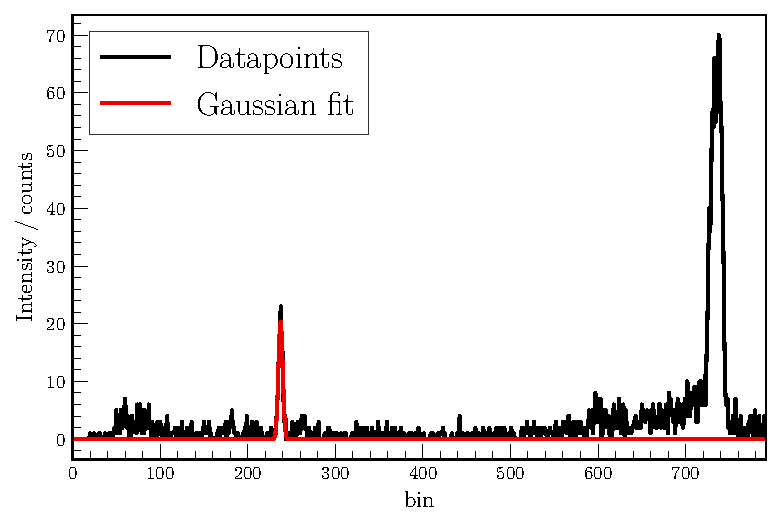
\includegraphics[width=\textwidth]{plots/GE-spectrum.pdf}
%     \caption{Spectrum of $\ce{Ge}$.}
% \end{subfigure}
% \begin{subfigure}{.3\textwidth}
%     \centering
%     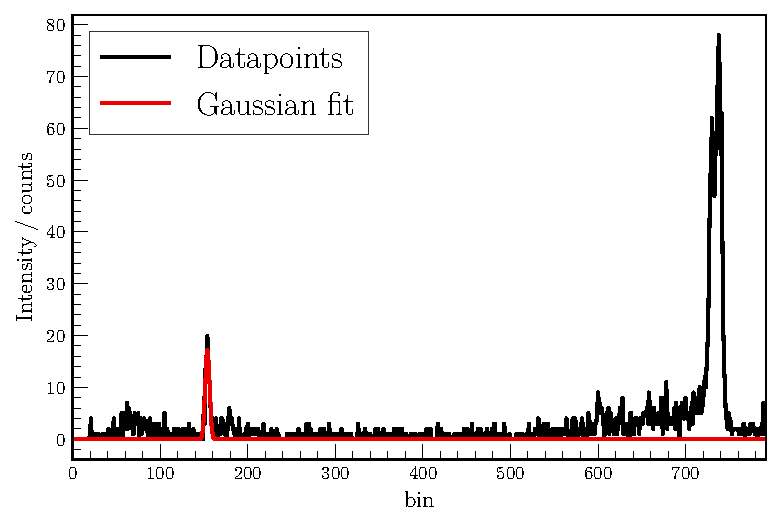
\includegraphics[width=\textwidth]{plots/FE-spectrum.pdf}
%   \caption{Spectrum of $\ce{Fe}$.}
% \end{subfigure}
% \caption{X-ray fluorescense spectra aquired by a MCA  A Gaussian fit is implemented around the characterisic emmision peak.}
% \end{figure*}

%%one figure inside the collums
% \begin{figure}
%     \captionsetup{width=0.9\linewidth}
%     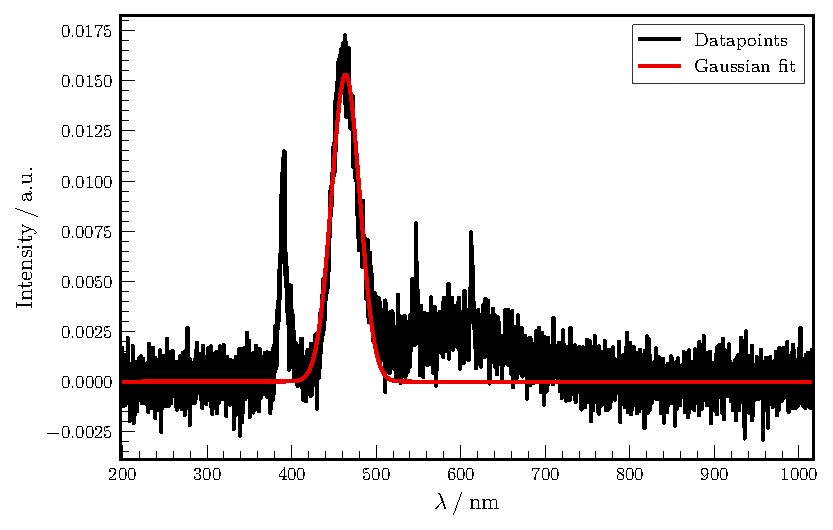
\includegraphics[width=0.5\textwidth]{plots/Samp_A_D.pdf}
%   \caption{Spectral measurement of sample A, excited by a UV-LED lightsource. A Gaussian fit of the peak contributed by luminescense is implemented.}
%     \label{fig:Samp_A_D}
% \end{figure}

\section{Results}
\label{sec:Results}

Here, the measurement data as well as the data proceeding is presented. 
Firstly, the x-ray fluorescence measuremnt is done, which corresponds to a compound analyzis.
Later, x-ray diffraction data, which have not been aquired by us are anayzed to get an estimation of the chemical bondings inside the unknown sample B.
\subsection{Energy scale}
\label{sec:scaling}

\begin{figure*}
    \centering
\begin{subfigure}{.3\textwidth}
    \centering
    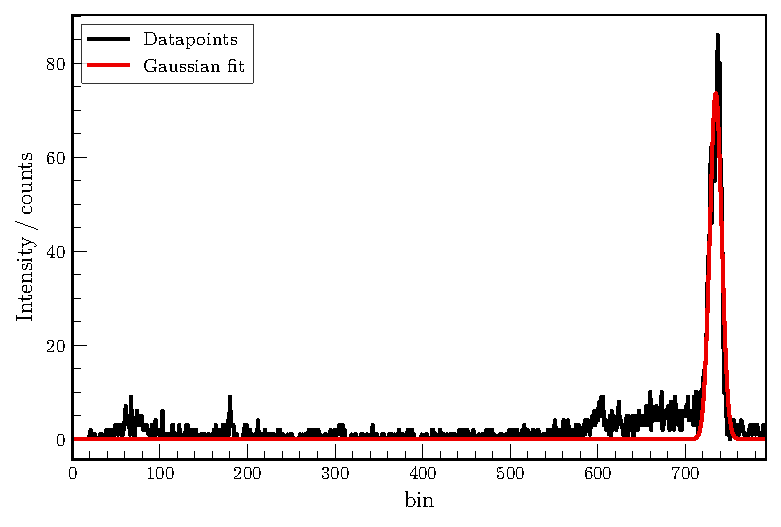
\includegraphics[width=\textwidth]{plots/source-spectrum.pdf}
    \caption{Spectrum of the source $\ce{Cs}$ due to the decay of $\ce{Br}$. }
\end{subfigure}
\begin{subfigure}{.3\textwidth}
    \centering
    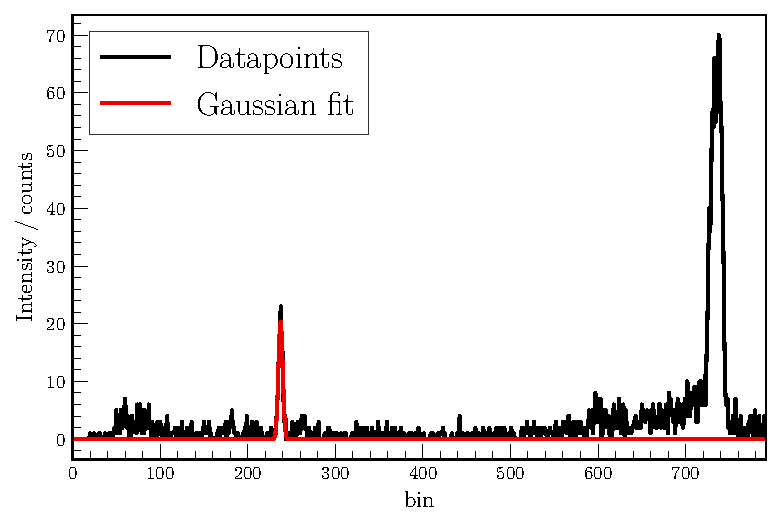
\includegraphics[width=\textwidth]{plots/GE-spectrum.pdf}
    \caption{Spectrum of $\ce{Ge}$.}
\end{subfigure}
\begin{subfigure}{.3\textwidth}
    \centering
    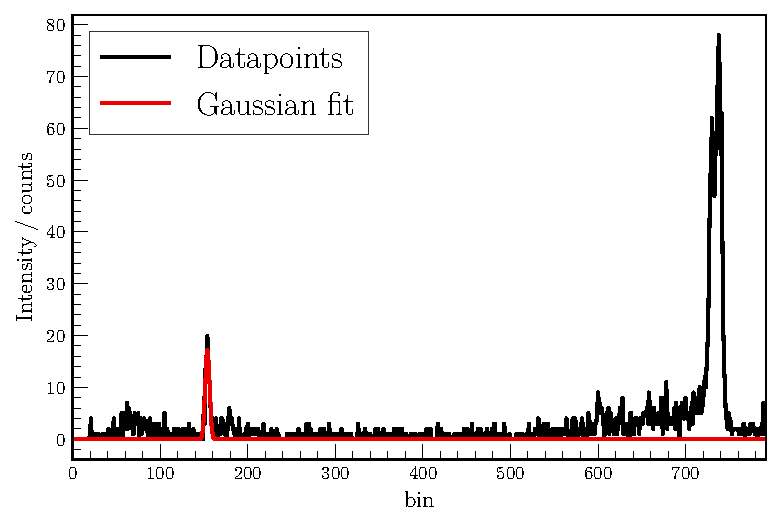
\includegraphics[width=\textwidth]{plots/FE-spectrum.pdf}
  \caption{Spectrum of $\ce{Fe}$.}
\end{subfigure}
\caption{X-ray fluorescene spectra aquired by a MCA. A Gaussian fit is implemented around the characterisic emission peak.}
\label{fig:scaling-samplesA}
\end{figure*}

\begin{figure*}
    \centering
\begin{subfigure}{.45\textwidth}
    \centering
    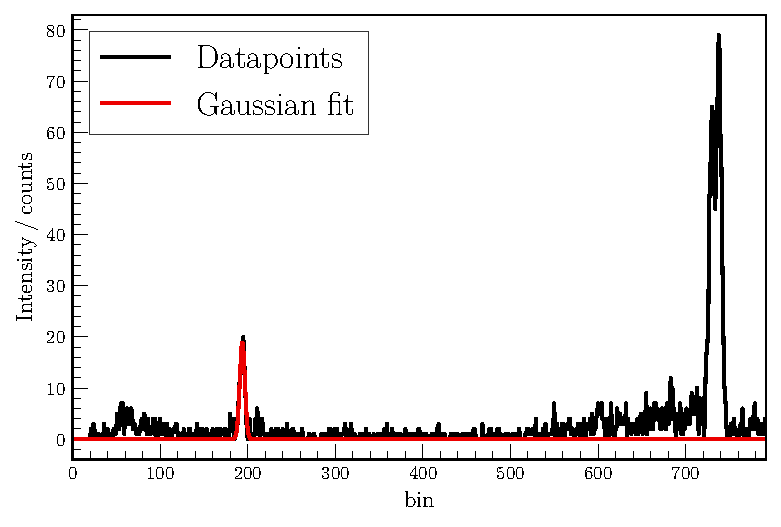
\includegraphics[width=\textwidth]{plots/Cu-spectrum.pdf}
    \caption{Spectrum of $\ce{Cu}$.}
\end{subfigure}
\begin{subfigure}{.45\textwidth}
    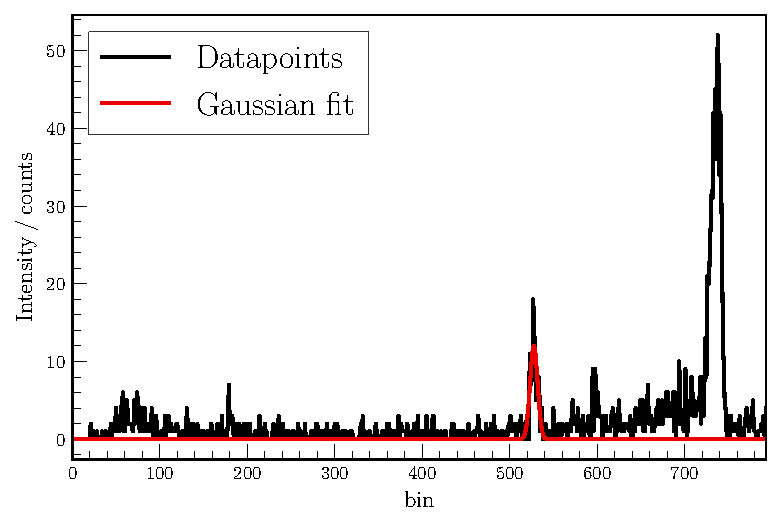
\includegraphics[width=\textwidth]{plots/Ag-spectrum.pdf}
  \caption{Spectrum of $\ce{Ag}$.}
\end{subfigure}
\caption{X-ray fluorescence spectra aquired by a MCA. A Gaussian fit is implemented around the characterisic emission peak.}
\label{fig:scaling-samplesB}
\end{figure*}

The spectra of the source $\ce{Cs}$, as well as the transmission spectra of $\ce{Ge}$,$\ce{Fe}$,$\ce{Cu}$ and $\ce{Ag}$ are given in figure \ref{fig:scaling-samplesA} and \ref{fig:scaling-samplesB}.
Also the spectrum of $\ce{Cr}$ has been measured, but the intensity of the characteristic spectrum is not efficient enough to refer a $\lambda_\text{peak}$.
The used value pairs are
\begin{table*}
    \caption{Characteristic \alpha line energy of several samples, listed with the bin of the MCA.}
    \label{tab:bin-E}
    \centering
    \begin{tabular}{l S[table-format=3.0] S[table-format=3.3]}
          \toprule
          {Material} & {Bin} & {$E \: [\si{\kilo\eV}]$} \\
          \midrule
          {Cs} & 735 & 30.972 \\
          {Ge} & 238 & 9.886  \\
          {Fe} & 154 & 6.407 \\
          {Cu} & 194 & 8.060 \\
          {Ag} & 528 & 22.163  \\
          \bottomrule
    \end{tabular}
\end{table*}
so that a linear regression function 
\begin{equation*}
    E(b) = (\SI{ 0.042 \pm 0.000 }{\kilo\eV}) \times b - (\SI{2.4 \pm 0.7}{\kilo\eV})
\end{equation*}
deduces, where $E$ is given in $keV$. 
This function is used to transform the bin scale into energy units in the following plots and calculations.

\subsection{Identifying sample B elements}
\label{sec:sampleB-fluo}

As done in section \ref{sec:scaling}, in the same way a x-ray-fluorescence measurement of the unknown sample B is done.
The resulting spectrum with the adopted energy scale is depicted in figure \ref{fig:Samp_B}. 
To delute the atomic composition of the sample, it is usefull to campare it with the $\alpha$-emmision lines of known samples.
Here, as it seems to fit very well, the primary emission lines of $\ce{Ni}$ and $\ce{Cu}$ are added to the plot.
As besides these to peaks, exept of the X-ray source peak around $\SI{30}{\kilo\eV}$ there is no other peak, one could derive the sample B is composed of $\ce{Ni}$ and $\ce{Cu}$.
To verify or adopt this analyzis, the X-ray diffraction spectrum can be taken into account in the following.

\begin{figure*}
    \centering
    \captionsetup{width=0.9\linewidth}
    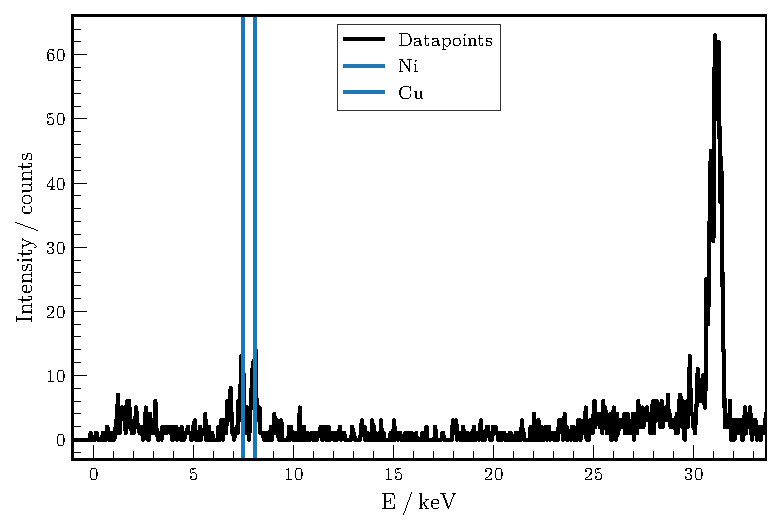
\includegraphics[width=0.8\textwidth]{plots/B-spectrum.pdf}
  \caption{Spectral measurement of sample B, excited by a x-ray due to $\ce{Cs}$ decay.The energy scale is created as given in chapter \ref{sec:scaling}. $\alpha$-line energies of $\ce{Ni}$ and $\ce{Cu}$ are implemented for comparision.}
    \label{fig:Samp_B}
\end{figure*}

\subsection{Identifying sample B chemical compunds}
\label{sec:sampleB-diff}

\begin{figure*}
    \centering
    \captionsetup{width=0.9\linewidth}
    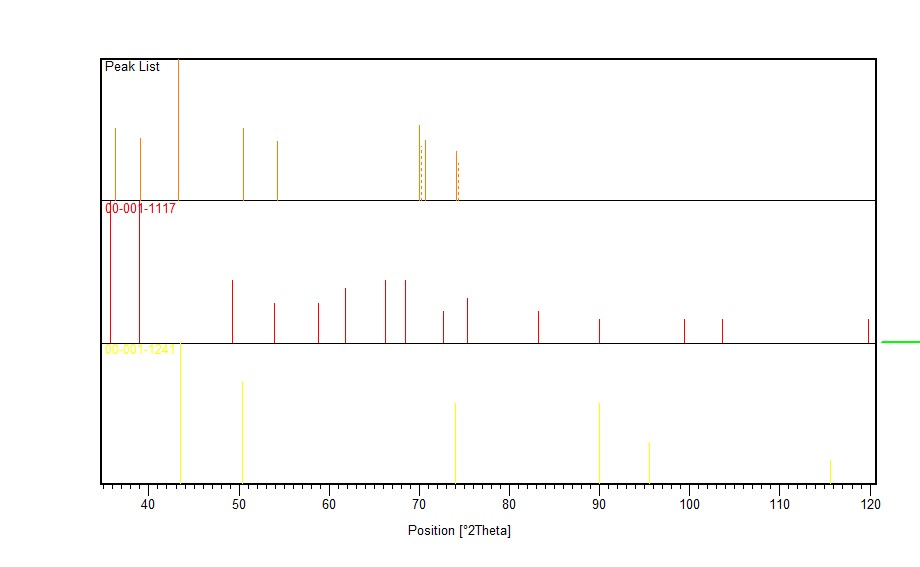
\includegraphics[width=0.8\textwidth]{graphics/SAMPLE_B_1.JPG}
  \caption{Spectral diffraction pattern of sample B (brown), excited by a x-ray due to $\ce{Cs}$ decay. For comparisson the diffraction pattern of $\ce{Cu}$\cite{Cu} (yellow) and $\ce{CuO}$\cite{CuO} (red) are added.)}
    \label{fig:diffraction}
\end{figure*}

As seen in figure \ref{fig:diffraction}, the diffraction spectrum of the measurement is given in intensity against angular position. 
The spectrum has been compared to several compounds of $\ce{Cu}$ $\ce{CuO}$, $\ce{Ni}$, $\ce{NiO}$ and $\ce{O}$ as these metals are the estimates from the fluorescence measurement \ref{sec:sampleB-fluo}.
The oxigen is added because the samples are not sealed and it is very likely it would have oxidized in the atmosphere.
What one could get from the comparission is, that the main peaks of the measurement can be related to the characteristic peaks of $\ce{Cu}$ \cite{Cu} and $\ce{CuO}$ \cite{CuO}.







